% A detailed introduction to the paper and concepts behind in
\section{Introduction} \label{sec:introduction}
In electrical and computer engineering, speed, power, and cost are the big three factors when it comes to designing processors. For decades, designers have been optimizing, analyzing, and testing the various trade-offs between the big three factors. Recently, processors have gained huge performance boosts, while memory access time has been mostly stagnant. This has led to the \emph{memory gap}\cite{Book}, as depicted in figure \ref{fig:memoryGap}. 

\begin{figure}[!htb]
    \centering
    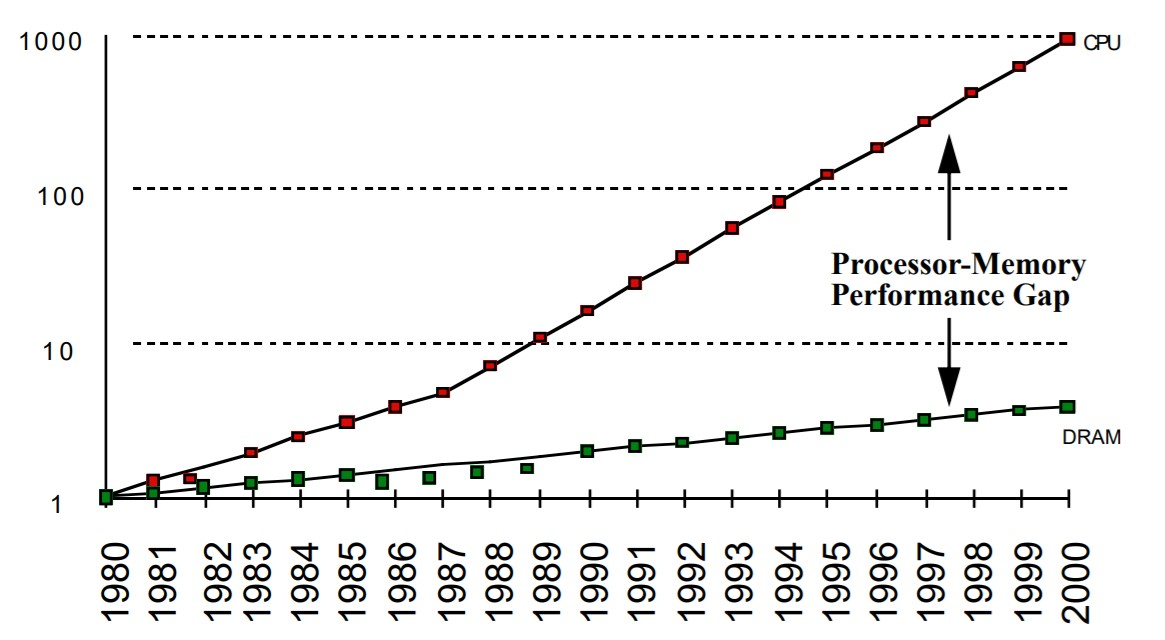
\includegraphics[width = 8cm]{images/memoryGap.jpg}
    \caption{Processor-Memory Performance Gap\cite{Book}.}
    \label{fig:memoryGap}
\end{figure}

To deal with the increasing difficulties of the memory gap, techniques such as multi-level caching and prefetching are becoming more important in modern-day computing.
In processor design, the cache is perhaps the most important when it comes to making optimizations. Because the processor requires massive amounts of data throughout the life of a program, optimizing cache performance has an astronomical impact on the efficiency of said processor. Some of those cache optimizations are done directly in the cache by modifying cache parameters such as block size, associativity, and cache size, or, by dividing the cache up into multiple levels of storage such as L1, L2, and sometimes L3. However, interior cache architecture isn't the only way to optimize miss ratios and latency times.

Prefetching\cite{Prefetch} is a method of fetching cache blocks before they are needed, in an effort to close the memory gap. This allows future cache blocks to be simultaneously moved into the cache, while a prior instruction is being executed. In order for a prefetcher to be effective, it must accomplish two things. It needs to be able to predict which blocks are going to be needed in the future, while ensuring that those blocks are in the cache early enough to reduce the latency time, however, not too early so the cache becomes polluted. Those prefetched blocks could be evicted, effectively ruining the entire point of the prefetcher.

In this paper we are going to explore two data prefetching algorithms known as Reference Prediction Table\cite{RPT} and Data-Correlating Prediction Table\cite{grannaes}. Because hardware is used to implement these prefetchers, the cost and power consumption may be slightly higher, but it's a trade-off that will be worth it for the increase in speed. Theoretically, if we could have an algorithm to perfectly predict the needed blocks of data, we could completely eliminate latency in our design. However, this isn't possible because we cannot predict the future with 100\% certainty. Because we do not have actual hardware to implement on, a hardware-simulator was used to simulate the prefetchers.

Following in the paper, section \ref{sec:background} will discuss a variety of prefetchers and their performance. The methods used in securing good results is explained in section \ref{sec:methodology}. The coding of the DCPT algorithm and its implementation is described in section \ref{sec:implementation}, and the results can be found in section \ref{sec:results}. Discussion, related work, and conclusion follows in sections \ref{sec:discussion}, \ref{sec:related-work}, \ref{sec:conclusion}, respectively.
